\chapter{Implementando Laboratório Virtual}\label{cap:proposta}

\section{Robot Operating System 2 (ROS2) e Gazebo 11}

O texto está bem escrito e claro, transmitindo informações importantes sobre o ROS e o ROS2. No entanto, sugiro fazer algumas pequenas alterações para melhorar a fluidez e a precisão:

O ROS, ou Robot Operating System, é uma plataforma de código aberto que fornece um conjunto de bibliotecas e ferramentas open-source para criar aplicações robóticas. Ele atua como um middleware entre a aplicação e os robôs, permitindo o controle de dispositivos em níveis baixos e a implementação de funcionalidades comuns, como troca de mensagens entre processos e gerenciamento de pacotes.

O ROS2 é a versão mais recente, projetada como uma evolução do ROS original, com melhorias significativas em áreas como segurança, escalabilidade, robustez e facilidade de uso. Ele suporta várias linguagens de programação, como C++, Python e outras, e oferece uma ampla gama de ferramentas e bibliotecas para auxiliar no desenvolvimento de software robótico.

Essas plataformas são fundamentais para o desenvolvimento de software robótico avançado, permitindo a criação de sistemas distribuídos e complexos, a reutilização de código e a integração com uma variedade de hardware e sensores.

No contexto do ROS, os conceitos de Node, Topic, Service e Action são essenciais para compreender como os sistemas robóticos são desenvolvidos e operam. Aqui está uma breve explicação de cada um:

\textbf{Node (Nó):} Um Node é um processo que executa uma função específica dentro de um sistema ROS. Os Nodes são unidades de processamento independentes que se comunicam uns com os outros por meio de mensagens. Cada Node pode realizar tarefas como controle de hardware, cálculos complexos, processamento de sensores, etc. Um sistema ROS geralmente consiste em vários Nodes que trabalham juntos para realizar tarefas complexas.

\textbf{Topic (Tópico):} Um Topic é um canal de comunicação assíncrono usado para enviar mensagens entre Nodes. Um Node pode publicar mensagens em um Topic e outro Node pode se inscrever para receber essas mensagens. Os Topics são usados para transmitir dados como leituras de sensores, comandos de controle, informações de estado, etc.

\textbf{Service (Serviço):} Um Service é uma forma de comunicação síncrona entre Nodes, onde um Node solicita um serviço a outro Node e aguarda a resposta. Os Services são usados para realizar operações que requerem uma resposta, como solicitar uma leitura de sensor específica, executar uma ação de controle, etc.

\textbf{Action (Ação):} As Actions são semelhantes aos Services, mas são usadas para operações que podem levar um tempo indeterminado para serem concluídas, como navegação de um robô até um determinado ponto. As Actions permitem que um Node envie uma solicitação, receba atualizações sobre o progresso da ação e, finalmente, receba uma resposta quando a ação for concluída.

Esses conceitos são fundamentais para o funcionamento do ROS, pois permitem que os Nodes se comuniquem de forma eficiente e realizem tarefas complexas de forma colaborativa em sistemas robóticos.

No ecossistema do ROS, RQT, RViz2 e Gazebo são componentes importantes que desempenham papéis distintos. Aqui está uma explicação de cada um:

\textbf{RQT:} O RQT é um framework de ferramentas gráficas para o ROS, que permite aos desenvolvedores visualizar e interagir com diferentes aspectos de um sistema ROS. Ele fornece uma variedade de plugins para tarefas como visualização de tópicos (\textit{topic}) e serviços (\textit{Service}), depuração, análise de dados, entre outros. O RQT é altamente extensível e pode ser personalizado para atender às necessidades específicas do desenvolvedor.

\textbf{RViz2:} O RViz2 é um visualizador 3D usado para exibir dados sensoriais, modelos de robôs, informações de navegação e outros dados relevantes em ambientes robóticos simulados ou reais. Ele permite que os desenvolvedores visualizem e interajam com o ambiente do robô de forma interativa, facilitando o desenvolvimento e depuração de algoritmos de controle e percepção.

\textbf{GAZEBO: }O Gazebo é um simulador robótico avançado que permite simular ambientes, sensores e atuadores com alta fidelidade. Ele é integrado ao ROS e é frequentemente usado para testar e validar algoritmos de controle em ambientes simulados antes de implantá-los em robôs reais. O Gazebo suporta a simulação de uma ampla variedade de sensores e atuadores, tornando-o uma ferramenta poderosa para o desenvolvimento de software robótico.

Essas ferramentas e conceitos são fundamentais para o desenvolvimento de sistemas robóticos com o ROS, fornecendo aos desenvolvedores as ferramentas necessárias para projetar, simular, visualizar e depurar seus sistemas robóticos de forma eficiente e eficaz.

No contexto do ROS (Robot Operating System) e do Gazebo, URDF (Unified Robot Description Format) e SDF (Simulation Description Format) são duas linguagens de marcação usadas para descrever modelos de robôs e ambientes de simulação, respectivamente. Aqui está uma explicação mais detalhada de cada um:

\textbf{URDF (Unified Robot Description Format):} O URDF é um formato de arquivo XML usado para descrever modelos de robôs em termos de suas estruturas, cinemática, visualização e outros aspectos relevantes para a simulação e controle. Ele é amplamente utilizado no ROS para descrever robôs em ambientes de simulação e no desenvolvimento de software de controle de robôs. O URDF permite especificar links, juntas, sensores, visualizações, entre outros componentes de um modelo de robô.

\textbf{SDF (Simulation Description Format):} O SDF é um formato de arquivo XML usado para descrever ambientes de simulação, incluindo modelos de robôs, objetos estáticos, luzes, terrenos e outras entidades. O SDF é usado principalmente no Gazebo, um simulador robótico popular, para definir o ambiente no qual os modelos de robôs são simulados. O SDF permite especificar a geometria, material, física e outras propriedades dos objetos no ambiente de simulação.

O URDF e o SDF são complementares e são frequentemente usados juntos no desenvolvimento de sistemas robóticos. O URDF descreve os modelos de robôs que serão controlados e simulados, enquanto o SDF descreve o ambiente no qual esses modelos serão colocados e interagirão. Juntos, esses formatos de arquivo permitem aos desenvolvedores criar simulações realistas de sistemas robóticos e testar seus algoritmos de controle em ambientes seguros e controlados antes de implantá-los em robôs reais.

O Gazebo é um simulador robótico avançado que suporta uma variedade de sensores usados em robôs. Ele oferece modelos precisos e realistas de sensores, permitindo que os desenvolvedores simulem o comportamento sensorial de seus robôs em ambientes virtuais. Alguns dos sensores comumente suportados pelo Gazebo incluem:

Câmeras: O Gazebo pode simular câmeras de diferentes tipos, como câmeras RGB, câmeras de profundidade e câmeras de infravermelho. Esses sensores podem ser usados para capturar imagens do ambiente do robô e são úteis para tarefas como navegação, reconhecimento de objetos e mapeamento.

Lidar: Lidar, ou Light Detection and Ranging, é um sensor usado para medir distâncias e gerar nuvens de pontos tridimensionais do ambiente. O Gazebo suporta diferentes tipos de sensores lidar, que são essenciais para aplicações como mapeamento, localização e evasão de obstáculos.

GPS: O Gazebo pode simular um receptor GPS, permitindo que os desenvolvedores testem algoritmos de localização global em seus robôs. O GPS é essencial para a navegação autônoma em ambientes externos.

IMU (Inertial Measurement Unit): Um IMU é um sensor que mede a aceleração e a taxa de rotação de um objeto. O Gazebo suporta a simulação de IMUs, que são usados para estimar a orientação e a velocidade angular de um robô.

O ROS 2 Control é um conjunto de ferramentas e bibliotecas no ROS 2 que facilita o controle de robôs. Ele fornece uma estrutura para implementar controladores de baixo nível para manipuladores, veículos e outros tipos de robôs. O ROS 2 Control suporta diferentes tipos de controladores, como controladores de posição, velocidade e esforço, e oferece recursos para configurar, ativar e desativar esses controladores de forma programática. Essa flexibilidade torna o ROS 2 Control adequado para uma variedade de aplicações robóticas, desde robôs industriais até veículos autônomos.

\section{Roteiro 0: Instalação e Configuração}
    
O presente projeto propõe o desenvolvimento de um laboratório virtual como de ambiente para o ensino de modelagem e controle de CubeSats por meio de simulação.
    
Utilizando ferramentas aberta e livres, contornando o problema de custo.

E de roteiros de instalação, configuração e uso, contornando o problema da curva de aprendizado.

Para a realização do presente projeto está foi escolhido as aplicações a seguir:

\begin{itemize}
    \item Ubuntu 22.04 LTS
    \item ROS 2 - Humble
    \item Gazebo 11
    \item GNU Octave
\end{itemize}

Para o funcionamento é previsto o hardware mínimo a seguir:

\begin{itemize}
    \item Memória: 4 GB
    \item Disco: SSD 120 GB
    \item Placa de Vídeo: 1GB Dedicada
    \item Processador: QuadCore 2.1 GHz
\end{itemize}

\subsection{Instalação ROS 2 Humble, Gazebo 11 Simulator e GNU Octave}

É possível encontrar o sistema operacional de forma gratuita pela pagina oficial do Ubuntu na referência \cite{ubuntuweb} e \cite{gazebosim}.

Faça a instalação mínima do sistema, abra o terminal pelo iniciar ou pelo comando de teclado, "CTRL+ALT+T". Selecione e cole a rotina abaixo para a instalação do ROS 2 Humble, o Gazebo 11 Simulator e o GNU Octave.

\begin{lstlisting}[language=bash,caption={bash version}]
#!/bin/bash

# Instala ROS

locale  # check for UTF-8

sudo apt update -y
sudo apt upgrade -y
sudo apt --fix-broken install -y
sudo apt autoremove -y

sudo apt install locales -y

sudo locale-gen en_US en_US.UTF-8
sudo update-locale LC_ALL=en_US.UTF-8 LANG=en_US.UTF-8
export LANG=en_US.UTF-8

locale  # verify settings

sudo apt install software-properties-common -y
sudo add-apt-repository universe -y

sudo apt update -y
sudo apt upgrade -y
sudo apt --fix-broken install -y
sudo apt autoremove -y

sudo apt install curl -y
sudo curl -sSL https://raw.githubusercontent.com/ros/rosdistro/master/ros.key -o /usr/share/keyrings/ros-archive-keyring.gpg

echo "deb [arch=$(dpkg --print-architecture) signed-by=/usr/share/keyrings/ros-archive-keyring.gpg] http://packages.ros.org/ros2/ubuntu $(. /etc/os-release && echo $UBUNTU_CODENAME) main" | sudo tee /etc/apt/sources.list.d/ros2.list > /dev/null

sudo apt update -y
sudo apt upgrade -y
sudo apt --fix-broken install -y
sudo apt autoremove -y

sudo apt install ros-humble-desktop -y
sudo apt install ros-dev-tools -y

source /opt/ros/humble/setup.bash
sudo apt install python3-pip -y
pip3 install -U argcomplete
pip3 install xacro
sudo apt install python3-colcon-common-extensions -y
echo "source /opt/ros/humble/setup.bash" >> ~/.bashrc


#ros2 run demo_nodes_cpp talker
#ros2 run demo_nodes_py listener

sudo apt install ros-humble-joint-state-publisher-gui
sudo apt install ros-humble-gazebo-ros-pkgs -y

sudo apt update -y
sudo apt upgrade -y
sudo apt --fix-broken install -y
sudo apt autoremove -y
\end{lstlisting}

Para testar a instalação abra duas abar no terminal e copie e cole:

\begin{lstlisting}[language=bash,caption={bash version}]
#!/bin/bash
ros2 run demo_nodes_cpp talker
\end{lstlisting}

Onde o resultado será:

[INFO] [1708993338.850590057] [talker]: Publishing: 'Hello World: 1'

[INFO] [1708993339.850601664] [talker]: Publishing: 'Hello World: 2'

Na primeira, e:

\begin{lstlisting}[language=bash,caption={bash version}]
#!/bin/bash
ros2 run demo_nodes_py listener
\end{lstlisting}

Na segunda, com o respectivo resultado sendo:

[INFO] [1708993347.861065131] [listener]: I heard: [Hello World: 10]

[INFO] [1708993348.851486479] [listener]: I heard: [Hello World: 11]

\subsection{Configuração ROS Package}

Abra o terminal, copie e cole a rotina abaixo:

\begin{lstlisting}[language=bash,caption={bash version}]
# Crie o diretorio
mkdir -p dev_ws/src
# Entre no diretorio
cd dev_ws
# Utilize o Colcon para construir seu Workspace
colcon build --symlink-install
# A flag symlink e usada por padrao
ls
#Verifice se as pastas build install log e src foram criadas, se sim, voce tem agora um workspace vazio.
# Os arquivos em ROS sempre sao organizados em packages, e eles devem estar no diretorio src
cd src
#Crie o package
ros2 pkg create --build-type ament_cmake my_package
# Crie a pasta Description Launcher e World
cd
mkdir -p dev_ws/src/my_package/description
mkdir -p dev_ws/src/my_package/launch
mkdir -p dev_ws/src/my_package/worlds
\end{lstlisting}

Com isso seu local de trabalho e pastas estão configuradas para trabalharmos com o ROS.

É recomendado, mas não obrigatório, usar um editor de código-fonte, por exemplo o GVim.

\section{Roteiro 1: Descrevendo CubeSat - Unified Robot Description Format}

No desenvolvimento de sistemas robóticos é desejado utilizar um linguagem comum para descrever o sistema. É interessante manter toda essa descrição no mesmo lugar onde outras aplicações fazem a referência, esse formato é o urdf. O arquivo urdf é formado por extruturas simples que se repetem ao longo do arquivo.

O primeiro passo é quebrar a estrutura do cubeSat em componentes separados que são chamados de \textit{links}. Para a separação dos \textit{links} tenha em mente o seguinte:

\begin{itemize}
    \item Se duas partes de movem independentemente entre elas, as mesmas precisam ser \textit{links} diferentes.
    \item Quando faz sentido a parte ser , ou faz algo além de se mover, \textit{e.g.}, como sensores.
\end{itemize}

Na escolha dos \textit{links} é necessário escolher sua origem, principalmente para partes que rotacionam pois esse será o ponto pivô.

Os links são definidos por três informações:

\begin{itemize}
    \item Visual: É o que vai ser visto no Gazebo.
    \begin{itemize}
        \item Geometria: Se refere ao formato
        \item Material: Se refere a cor
    \end{itemize}
    \item Collision: Usa os valores anteriores, mas determina a fronteira de interação entre links. 
    \item Inertial: Todas as propriedades inerciais.
    \begin{itemize}
        \item Massa: A massa do objeto
        \item Inercia: A matriz de inercia do objeto
    \end{itemize}
\end{itemize}

Como no exemplo a seguir de um paralelepípedo arbitrário a seguir:

\begin{lstlisting}[language=XML,caption={XML version}]
    <link name="NOME_link">
        <visual>
            <origin xyz="0 0 0" rpy="0 0 0"/>
            <geometry>
                <box size="${Aresta_X} ${Aresta_Y} ${Aresta_Z}" />
            </geometry>
            <material name="blue"/>
        </visual>
        <collision>
            <origin xyz="0 0 0" rpy="0 0 0"/>
            <geometry>
                <box size="${Aresta_X} ${Aresta_Y} ${Aresta_Z}" /
            </geometry>
        </collision>
        <inertial>
            <origin xyz="0 0 0" rpy="0 0 0"/>
            <mass value="${MASSA}" />
            <inertia
                ixx="Ixx" ixy="0.0" ixz="0.0"
                iyy="Iyy" iyz="0.0"
                izz="Izz" />
            </inertial>
        </link>
\end{lstlisting}


Agora devemos definir as relações entre esses \textit{links}, essa relação é definida pelas \textit{joints}, relacionando assim o movimento, rotação entre os sistemas de coordenadas de cada link, por isso em sua descrição é necessário dizer o tipo de movimento que está usando.

As \textit{joints} são descritas por:

\begin{itemize}
    \item Tipo:
    \begin{itemize}
        \item Revolução, Continua, Fixa, Flutuante...
    \end{itemize}
    \item \textit{Parent Link}
    \item \textit{Child Link}
    \item Origem, eixos de movimento, e limites.
\end{itemize}

Como no exemplo de uma junta continua, caracteriza o movimento de rotação entre dois \textit{links}, em relação ao eixo z do \textit{link pai}:

\begin{lstlisting}[language=XML,caption={XML version}]
<joint name="NOME_joint" type="continuous">
<origin xyz="0 0 0" rpy="0 0 0"/>
<parent link="Nome_link_Pai"/>
<child link="Nome_link_filho"/>
<axis xyz ="0 0 1" rpy = "0 0 0"/>
<limit effort="10000" velocity="10000"/>
<joint_properties damping ="0.0" friction="0.0"/>
</joint>
\end{lstlisting}

\subsubsection{Descrição do CubeSat}

\begin{lstlisting}[language=XML,caption={XML version}]
<?xml version="1.0"?>
<robot xmlns:xacro="http://www.ros.org/wiki/xacro"  name="robot">

    <link name="world"></link>
    
    <joint name="1U_joint" type="floating">
    	<origin xyz="0 0 0" rpy="0 0 0"/>
    	<parent link="world"/>
    	<child link="1U_link"/>
    </joint>

    <xacro:property name="U_aresta" value="0.1" />
    <xacro:property name="U_massa" value="1" />
    
    <link name="1U_link">
        <visual>
            <origin xyz="0 0 0" rpy="0 0 0"/>
            <geometry>
                <box size="${U_aresta} ${U_aresta} ${U_aresta}" />
            </geometry>
	 <material name="blue"/>
        </visual>
        <collision>
            <origin xyz="0 0 0" rpy="0 0 0"/>
            <geometry>
                <box size="${U_aresta} ${U_aresta} ${U_aresta}" />
            </geometry>
        </collision>
        <inertial>
            <origin xyz="0 0 0" rpy="0 0 0"/>
            <mass value="${U_massa}" />
            <inertia ixx="${(1/12) * U_massa * (U_aresta*U_aresta+U_aresta*U_aresta)}" ixy="0.0" ixz="0.0"
                    iyy="${(1/12) * U_massa * (U_aresta*U_aresta+U_aresta*U_aresta)}" iyz="0.0"
                    izz="${(1/12) * U_massa * (U_aresta*U_aresta+U_aresta*U_aresta)}" />
        </inertial>
    </link>

    <joint name="2U_joint" type="fixed">
        <origin xyz="0 0 ${U_aresta/2} " rpy="0 0 0"/>
        <parent link="1U_link"/>
        <child link="2U_link"/>
    </joint>

    <link name="2U_link">
        <visual>
            <origin xyz="0 0 ${U_aresta/2}" rpy="0 0 0"/>
            <geometry>
                <box size="${U_aresta} ${U_aresta} ${U_aresta}" />
            </geometry>
		<material name="orange"/>
        </visual>
        <collision>
            <origin xyz="0 0 ${U_aresta/2}" rpy="0 0 0"/>
            <geometry>
                <box size="${U_aresta} ${U_aresta} ${U_aresta}" />
            </geometry>
        </collision>
        <inertial>
            <origin xyz="0 0 ${U_aresta/2}" rpy="0 0 0"/>
            <mass value="${U_massa}" />
            <inertia ixx="${(1/12) * U_massa * (U_aresta*U_aresta+U_aresta*U_aresta)}" ixy="0.0" ixz="0.0"
                    iyy="${(1/12) * U_massa * (U_aresta*U_aresta+U_aresta*U_aresta)}" iyz="0.0"
                    izz="${(1/12) * U_massa * (U_aresta*U_aresta+U_aresta*U_aresta)}" />
        </inertial>
    </link>
    
    <joint name="3U_joint" type="fixed">
        <origin xyz="0 0 ${U_aresta}" rpy="0 0 0"/>
        <parent link="2U_link"/>
        <child link="3U_link"/>

    </joint>

    <link name="3U_link">
        <visual>
            <origin xyz="0 0 ${U_aresta/2}" rpy="0 0 0"/>
            <geometry>
                <box size="${U_aresta} ${U_aresta} ${U_aresta}" />
            </geometry>
		<material name="green"/>
        </visual>
        <collision>
            <origin xyz="0 0 ${U_aresta/2}" rpy="0 0 0"/>
            <geometry>
                <box size="${U_aresta} ${U_aresta} ${U_aresta}" />
            </geometry>
        </collision>
        <inertial>
            <origin xyz="0 0 ${U_aresta/2}" rpy="0 0 0"/>
            <mass value="1" />
            <inertia ixx="${(1/12) * U_massa * (U_aresta*U_aresta+U_aresta*U_aresta)}" ixy="0.0" ixz="0.0"
                    iyy="${(1/12) * U_massa * (U_aresta*U_aresta+U_aresta*U_aresta)}" iyz="0.0"
                    izz="${(1/12) * U_massa * (U_aresta*U_aresta+U_aresta*U_aresta)}" />
        </inertial>
    </link>

    <joint name="camera_joint" type="fixed">
        <origin xyz="${U_aresta} 0 ${U_aresta/2}" rpy="0 0 0"/>
        <parent link="3U_link"/>
        <child link="camera_link"/>        
    </joint>

    <link name="camera_link">
        <visual>
            <origin xyz="0 0 0" rpy="0 0 0"/>
            <geometry>
                <box size="${U_aresta} ${U_aresta} ${U_aresta}" />
            </geometry>
		<material name="white"/>
        </visual>
        <collision>
            <origin xyz="0 0 0" rpy="0 0 0"/>
            <geometry>
                <box size="${U_aresta} ${U_aresta} ${U_aresta}" />
            </geometry>
        </collision>
        <inertial>
            <origin xyz="0 0 0" rpy="0 0 0"/>
            <mass value="1" />
            <inertia ixx="${(1/12) * U_massa * (U_aresta*U_aresta+U_aresta*U_aresta)}" ixy="0.0" ixz="0.0"
                    iyy="${(1/12) * U_massa * (U_aresta*U_aresta+U_aresta*U_aresta)}" iyz="0.0"
                    izz="${(1/12) * U_massa * (U_aresta*U_aresta+U_aresta*U_aresta)}" />
        </inertial>
    </link>

    <joint name="5U_joint" type="fixed">
        <origin xyz="${U_aresta} 0 ${U_aresta/2}" rpy="0 0 0"/>
        <parent link="2U_link"/>
        <child link="5U_link"/>
    </joint>

    <link name="5U_link">
        <visual>
            <origin xyz="0 0 0" rpy="0 0 0"/>
            <geometry>
                <box size="${U_aresta} ${U_aresta} ${U_aresta}" />
            </geometry>
		<material name="gray"/>
        </visual>
        <collision>
            <origin xyz="0 0 0" rpy="0 0 0"/>
            <geometry>
                <box size="${U_aresta} ${U_aresta} ${U_aresta}" />
            </geometry>
        </collision>
        <inertial>
            <origin xyz="0 0 0" rpy="0 0 0"/>
            <mass value="1" />
            <inertia ixx="${(1/12) * U_massa * (U_aresta*U_aresta+U_aresta*U_aresta)}" ixy="0.0" ixz="0.0"
                    iyy="${(1/12) * U_massa * (U_aresta*U_aresta+U_aresta*U_aresta)}" iyz="0.0"
                    izz="${(1/12) * U_massa * (U_aresta*U_aresta+U_aresta*U_aresta)}" />
        </inertial>
    </link>    
    
        <joint name="6U_joint" type="fixed">
        <origin xyz="${U_aresta} 0 0" rpy="0 0 0"/>
        <parent link="1U_link"/>
        <child link="6U_link"/>
    </joint>

    <link name="6U_link">
        <visual>
            <origin xyz="0 0 0" rpy="0 0 0"/>
            <geometry>
                <box size="${U_aresta} ${U_aresta} ${U_aresta}" />
            </geometry>
		<material name="gray"/>
        </visual>
        <collision>
            <origin xyz="0 0 0" rpy="0 0 0"/>
            <geometry>
                <box size="${U_aresta} ${U_aresta} ${U_aresta}" />
            </geometry>
        </collision>
        <inertial>
            <origin xyz="0 0 0" rpy="0 0 0"/>
            <mass value="1" />
            <inertia ixx="${(1/12) * U_massa * (U_aresta*U_aresta+U_aresta*U_aresta)}" ixy="0.0" ixz="0.0"
                    iyy="${(1/12) * U_massa * (U_aresta*U_aresta+U_aresta*U_aresta)}" iyz="0.0"
                    izz="${(1/12) * U_massa * (U_aresta*U_aresta+U_aresta*U_aresta)}" />
        </inertial>
    </link> 
    <xacro:include filename="example_gazebo.xacro" />

</robot>
\end{lstlisting}

Itens para evitar repetição como propriedades e macros para incluir

\begin{lstlisting}[language=XML,caption={XML version}]
<?xml version="1.0"?>
<robot xmlns:xacro="http://www.ros.org/wiki/xacro" >

    <material name="white">
        <color rgba="1 1 1 1"/>
    </material>

    <material name="gray">
        <color rgba="0.3 0.3 0.3 1"/>
    </material>

    <material name="orange">
        <color rgba="1 0.3 0.1 1"/>
    </material>

    <material name="blue">
        <color rgba="0.2 0.2 1 1"/>
    </material>

    <material name="green">
        <color rgba="0.2 1 0.2 1"/>
    </material>

    <xacro:macro name="inertial_sphere" params="mass radius *origin">
        <inertial>
            <xacro:insert_block name="origin"/>
            <mass value="${mass}" />
            <inertia ixx="${(2/5) * mass * (radius*radius)}" ixy="0.0" ixz="0.0"
                    iyy="${(2/5) * mass * (radius*radius)}" iyz="0.0"
                    izz="${(2/5) * mass * (radius*radius)}" />
        </inertial>
    </xacro:macro>  

    <xacro:macro name="inertial_box" params="mass x y z *origin">
        <inertial>
            <xacro:insert_block name="origin"/>
            <mass value="${mass}" />
            <inertia ixx="${(1/12) * mass * (y*y+z*z)}" ixy="0.0" ixz="0.0"
                    iyy="${(1/12) * mass * (x*x+z*z)}" iyz="0.0"
                    izz="${(1/12) * mass * (x*x+y*y)}" />
        </inertial>
    </xacro:macro>


    <xacro:macro name="inertial_cylinder" params="mass length radius *origin">
        <inertial>
            <xacro:insert_block name="origin"/>
            <mass value="${mass}" />
            <inertia ixx="${(1/12) * mass * (3*radius*radius + length*length)}" ixy="0.0" ixz="0.0"
                    iyy="${(1/12) * mass * (3*radius*radius + length*length)}" iyz="0.0"
                    izz="${(1/2) * mass * (radius*radius)}" />
        </inertial>
    </xacro:macro>

</robot>
\end{lstlisting}

Configurações adicionais para o gazebo

\begin{lstlisting}[language=XML,caption={XML version}]
<?xml version="1.0"?>
<robot xmlns:xacro="http://www.ros.org/wiki/xacro">

    <gazebo reference="1U_link">
        <material>Gazebo/Blue</material>
    </gazebo>

    <gazebo reference="2U_link">
        <material>Gazebo/Orange</material>
    </gazebo>

    <gazebo reference="3U_link">
        <material>Gazebo/Green</material>
    </gazebo>

    <gazebo reference="5U_link">
        <material>Gazebo/Gray</material>
    </gazebo>
    
    <gazebo reference="ADCS_link">
        <material>Gazebo/Gray</material>
    </gazebo>

    <gazebo>
        <plugin name="gazebo_ros_joint_state_publisher"
            filename="libgazebo_ros_joint_state_publisher.so">
            <update_rate>20</update_rate>
            <joint_name>1U_joint</joint_name>
        </plugin>
    </gazebo>

    <gazebo>
	<plugin filename="gz-sim-imu-system"
        name="gz::sim::systems::Imu">
             <update_rate>20</update_rate>
            <joint_name>1U_joint</joint_name>
	</plugin>
    </gazebo>

    <gazebo>
        <plugin name="gazebo_ros_joint_pose_trajectory"
            filename="libgazebo_ros_joint_pose_trajectory.so">
            <update_rate>2</update_rate>
                <joint_name>1U_joint</joint_name>
        </plugin>
    </gazebo>

</robot>
\end{lstlisting}



\begin{figure}[htpb]
\centering
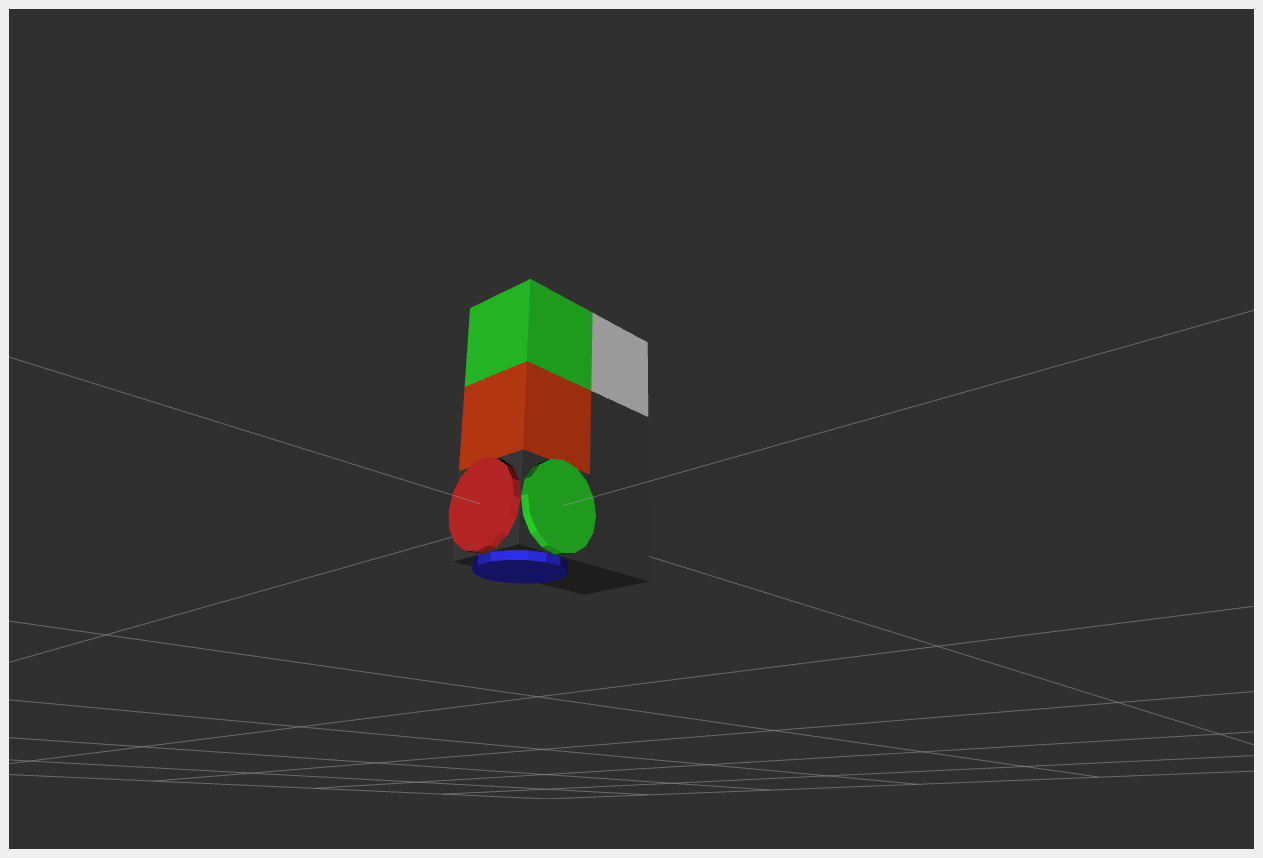
\includegraphics[scale=0.3]{figs/rviz_screenshot_2024_04_08-19_21_06.png}
\caption{Vizualização ROS2 do URDF do CUBESAT 6U}
\label{fig:12}
\end{figure}

\section{Roteiro 2: Adicionando Sensores -  Gazebo Pluggins}

\subsection{Sensor IMU}

O IMU (Inertial Measurement Unit) Gazebo Sensor é uma ferramenta crucial na simulação de robôs em ambientes virtuais, como o Gazebo. Ele simula sensores que medem a orientação e a aceleração do robô, fornecendo dados importantes para a navegação e controle. Com o IMU, é possível testar algoritmos de fusão sensorial, odometria e controle de forma precisa e eficaz, sem a necessidade de hardware real. Isso torna o desenvolvimento e a depuração de sistemas robóticos mais acessíveis e econômicos.

Ele é adicionado da seguinte maneira:

\begin{lstlisting}[language=XML,caption={XML version}]
    <joint name="6U_ADCS_joint" type="fixed">
        <origin xyz="0 0 0" rpy="-1.571 0 -1.571" />
        <parent link="6U_link" />
        <child link="6U_ADCS_link" />
    </joint>

    <link name="6U_ADCS_link"></link>
    
    <gazebo reference="6U_link">
	<sensor name="imu_sensor" type="imu">
    		<always_on>1</always_on>
    		<update_rate>1</update_rate>
    		<visualize>true</visualize>
    		<topic>imu</topic>
	</sensor>
    </gazebo>
\end{lstlisting}

Os dados do IMU são orientação, velocidade angular e aceleração linear. A saída das mensagens enviadas sobre o tópico /imu deve se assemelhar com o seguinte:

\begin{lstlisting}[language=bash,caption={Bash version}]
    ---
header:
  stamp:
    sec: 393
    nanosec: 424000000
  frame_id: 1U_link
orientation:
  x: 0.023725517648530682
  y: 0.04281485544486788
  z: -0.48399201528223695
  w: 0.8737023046258853
orientation_covariance:
- 0.0
- 0.0
- 0.0
- 0.0
- 0.0
- 0.0
- 0.0
- 0.0
- 0.0
angular_velocity:
  x: -0.05568477597832236
  y: -0.020611977578691595
  z: 0.2085619814357944
angular_velocity_covariance:
- 0.0
- 0.0
- 0.0
- 0.0
- 0.0
- 0.0
- 0.0
- 0.0
- 0.0
linear_acceleration:
  x: -0.3077501933465464
  y: -0.6085366879098204
  z: 10.27332940477441
linear_acceleration_covariance:
- 0.0
- 0.0
- 0.0
- 0.0
- 0.0
- 0.0
- 0.0
- 0.0
- 0.0
---
\end{lstlisting}

\subsection{Sensor Câmera}

A adição do plugin de câmera no Gazebo é fundamental para simulações que requerem visão computacional ou processamento de imagens. Esse plugin permite a simulação de câmeras em um ambiente virtual, gerando imagens realistas que podem ser processadas por algoritmos de visão computacional.

Ao adicionar o plugin de câmera, é possível configurar diversos parâmetros, como resolução da imagem, campo de visão, tipo de lente, entre outros. Além disso, o plugin permite que as imagens geradas sejam publicadas em tópicos ROS, facilitando a integração com outros componentes do sistema robótico virtual.

Com a adição do plugin de câmera, os desenvolvedores podem testar e depurar algoritmos de visão computacional em um ambiente controlado e seguro, antes de implementá-los em hardware real. Isso acelera o desenvolvimento de sistemas robóticos que dependem de percepção visual, como robôs autônomos e sistemas de monitoramento.

            
\begin{lstlisting}[language=XML,caption={XML version}]
    <joint name="camera_optical_joint" type="fixed">
        <origin xyz="0 0 0" rpy="-1.571 0 -1.571" />
        <parent link="camera_link" />
        <child link="camera_link_optical" />
    </joint>

    <link name="camera_link_optical"></link>

    <gazebo reference="camera_link">
        <sensor type="depth" name="my_camera">
            <update_rate>20</update_rate>
            <visualize>true</visualize>
            <camera name="cam">
                <horizontal_fov>1.3962634</horizontal_fov>
                <image>
                    <width>640</width>
                    <height>480</height>
                    <format>R8B8G8</format>
                </image>
                <clip>
                    <near>0.02</near>
                    <far>300</far>
                </clip>
                <noise>
                    <type>gaussian</type>
                    <mean>0.0</mean>
                    <stddev>0.007</stddev>
                </noise>
            </camera>
            <plugin name="camera_controller" filename="libgazebo_ros_camera.so">
                <frame_name>camera_link_optical</frame_name>
                <min_depth>0.1</min_depth>
                <max_depth>500</max_depth>
            </plugin>
        </sensor>
    </gazebo>
\end{lstlisting}


\begin{figure}[htpb]
\centering
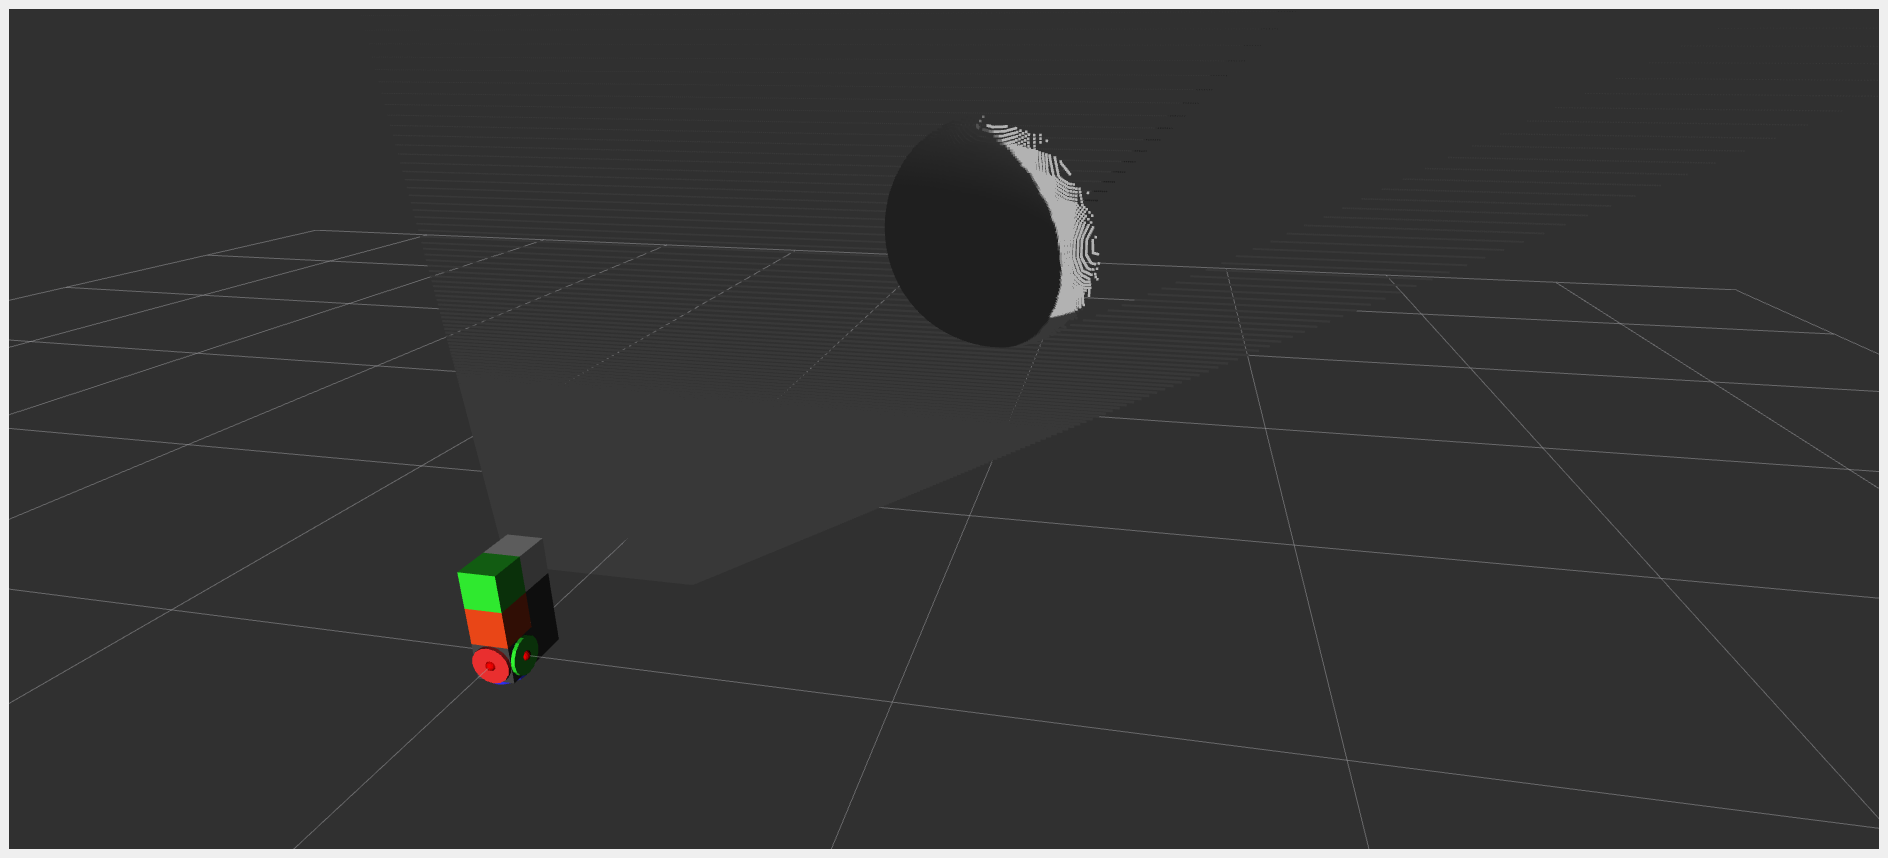
\includegraphics[scale=0.3]{figs/rviz_screenshot_camera_2024_04_08-19_34_54.png}
\caption{Point Cloud do Sensor Câmera Visualização ROS2 do URDF do CUBESAT 6U}
\label{fig:12}
\end{figure}

\section{Considerações Finais}

Ao longo desta dissertação, exploramos o potencial do ROS 2 e do simulador Gazebo 11 para a modelagem e simulação de um CubeSat, assim como seu ambiente operacional em órbita baixa. A utilização destas ferramentas se mostrou altamente promissora, oferecendo um ambiente robusto e flexível para o desenvolvimento de sistemas espaciais.

A integração de sensores de câmera e IMU no simulador foi relativamente simples, permitindo a simulação de dados sensoriais realistas para o CubeSat virtual. Estes sensores são fundamentais para as operações de um satélite, incluindo orientação, navegação e controle.

Por outro lado, a implementação do ROS 2 Control tem sido um desafio significativo. A transição do ROS 1 para o ROS 2 e a adaptação aos novos padrões de controle têm exigido um esforço adicional de desenvolvimento e depuração. No entanto, a utilização do ROS 2 Control oferece benefícios a longo prazo, como maior eficiência e suporte aprimorado para sistemas distribuídos.

A representação precisa do ambiente em órbita baixa também se mostra desafiadora. A modelagem de fenômenos como arrasto atmosférico, perturbações gravitacionais e interações com outros corpos celestes requer um esforço adicional de pesquisa e desenvolvimento. No entanto, a precisão deste ambiente é crucial para a validação dos sistemas de controle e navegação do CubeSat.

Em suma, o uso do ROS 2 e do Gazebo Simulator 11 para a modelagem e simulação de um CubeSat e seu ambiente operacional em órbita baixa é altamente promissor, apesar dos desafios encontrados. Estas ferramentas oferecem um ambiente rico e flexível para o desenvolvimento e teste de sistemas espaciais, contribuindo para o avanço da tecnologia espacial.
